\newpage
\genHeader

\section{Load a Simple Demo}

Did you notice the headings changed again? If you did, awesome! If not, we must emphasize viewing this handbook double sided so that you don't miss any future changes.

\begin{itemize}
\item[$\blacktriangleright$] Open up Eclipse with a clean, fresh workspace. Go to ``Window/Open Perspective/Other\ldots'' \footnote{A path given as ``foo/bar'' indicates how to navigate in a series of menus and submenus.} and choose eMoflon~(Fig.~\ref{fig_eclipse}).

\begin{figure}[htbp]
	\centering
  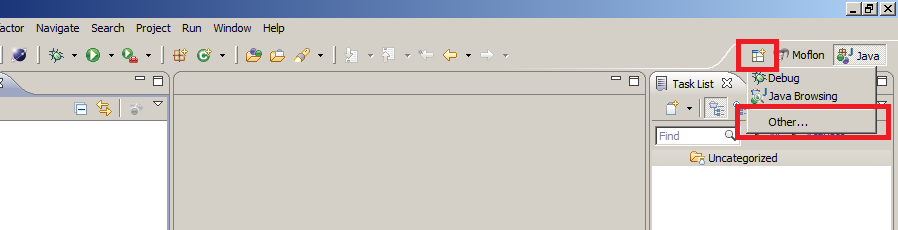
\includegraphics[width=\textwidth]{eclipse_firststart}
	\caption{Choose the eMoflon perspective.}
	\label{fig_eclipse}
\end{figure} 

\item[$\blacktriangleright$] At either the far right or center of the toolbar, a new action set should have appeared. Choose ``New Metamodel'' (Fig.~\ref{fig_eclipseNewMetamodelButton}).
\footnote{The button with an `L' shows you our logfile (important input for us if something goes wrong!). You remember our email address, right?}

\begin{figure}[htbp]
	\centering
  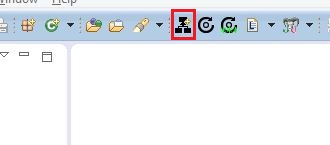
\includegraphics[width= 0.8\textwidth]{eclipse_newMetamodelButton}
	\caption{Eclipse ''New Metamodel''}
	\label{fig_eclipseNewMetamodelButton}
\end{figure}

\item[$\blacktriangleright$] A new dialog box should appear. This is the place where you officially decide which eMoflon syntax you'd like to use (Fig.~\ref{fig_chooseSyntax}). There's no advantage to using one over the other; the decision is purely preferential. With visual, you'll be using Eclipse alongside the EA program you just installed. You'll use EA to build several kinds of diagrams, then refresh and run the program using eclipse. With textual (MOSL), you'll be editing and running the project entirely within the Eclipse IDE. No matter which syntax you choose however, name your project ``Demo'' and make sure the `Add Demo Specification' button is checked off. This will build all the files and tests required to ensure you've set up the program correctly.  

\vspace{1cm}

\begin{figure}[htbp]
	\centering
  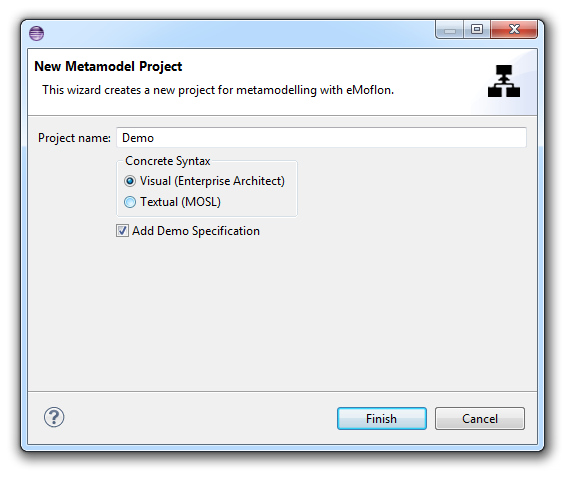
\includegraphics[width=\textwidth]{eclipse_newMetamodelDialog}
	\caption{Choose your syntax}
	\label{fig_chooseSyntax}
\end{figure} 
\end{itemize}

\newpage
\visHeader

\begin{itemize}
\FloatBarrier
\item[$\blacktriangleright$] Did you notice the new Demo.eap file in your package explorer? This is the EA file you'll be testing and modelling your program with. Don't worry about the other folder and the exclamation mark it carries. The problems will be resolved by the end of this page.

In the meantime, Please do not rename, move, or delete anything.

\item[$\blacktriangleright$] Double click ``Demo.eap'' to start EA, and choose ``Ultimate" when starting EA for the first time.

\item[$\blacktriangleright$] In EA, choose ``Extensions/MOFLON::Ecore Addin/Export\- all\- to\- Workspace'' (Fig.~\ref{fig_ea}).

\vspace{1cm}

\begin{figure}[htbp]
	\centering
  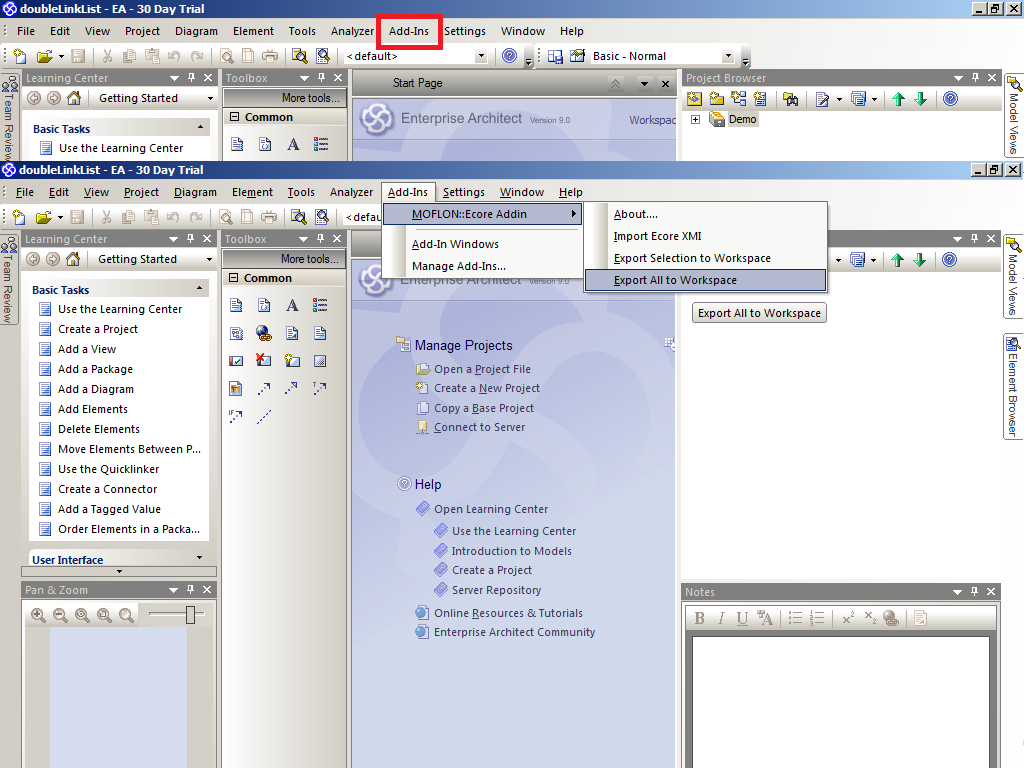
\includegraphics[width=0.9\textwidth]{ea_firststart}
	\caption{Export from EA using our extension} 
	\label{fig_ea} 
\end{figure}

\vspace{1cm}

\item[$\blacktriangleright$] Now try exploring the project browser! Try to navigate and understand some of the files and diagrams. This simple demo is meant to familiarize you with visual representations classes, functions, and how they relate to eMoflon's generated code. Don't worry if you get confused - we provide plenty of help and references throughout the tutorial.
  
\item[$\blacktriangleright$] Switch back to Eclipse, choose your Metamodel project, and press F5 to refresh. A new folder should appear, and your errors should disappear after a few seconds. Since you've chosen to use the Visual Syntax, there isn't much to look at here. The export from EA places all required files in a hidden folder in the project, and refreshing triggers a build process that invokes our code generators automatically. 
You should be able to monitor the progress with the green bar in the lower right corner. Pressing the symbol opens a monitor view that gives more details of the build process. You don't need to worry about any of these details, just remember to refresh your Eclipse workspace after an export.

\end{itemize}

\newpage
\texHeader

Now, lets think about this whole Text Syntax. How exactly does it work? How will we be able to generate Java code from our simplified model code?

As you now know, Emoflon is an plug-in tool for Eclipse. More precisely, EMoflon needs the the Eclipse Modeling Framework (EMF) in order to work. EMF is comprised of two separate Metamodels - Genmodel and Ecore. The Genmodel contains the boring information about code generation like path and file information. 
We are more interested in Ecore, which we represent through our MOSL syntax. 

When you switched the project explorer from ``Projects" to ``Top Level Elements," you noticed that a few new nodes were created. Each node you see has a different criteria for grouping related Eclipse Projects together, which makes them your project ``Working Sets.'' The ``Specification'' node contains all the metamodels projects in a workspace (Fig. ~\ref{fig_modelSpecification}). That means, for every new Metamodel you create in your current workspace, all of the text code will be placed here. 

 \begin{figure}[htbp]
  \centering
  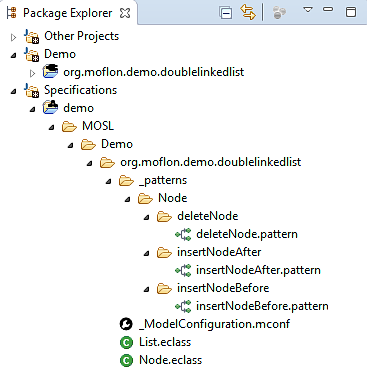
\includegraphics[width=0.5\textwidth]{eclipse_Specification}
  \caption{Eclipse: Specification Working Set}
  \label{fig_modelSpecification}
\end{figure}
  

Instead, lets look at the two eclass files and their syntax. Expand the folders, and you'll see that each eclass is declared in its own file. While you can combine several class delcarations in a single file in some languages (like Java), with MOSL it really is best to have them separated. It'll all make sense in a moment when we discuss Patterns.

Inspect the ``List'' class, and you'll see it has a just one EAttribute. EAttributes are defined by their name followed by a colon symbol and type.
This class also has a container reference represented by the diamond operator in front of an arrow.
The second reference type is a simple reference which